\section{Methods}

\subsection{Variational auto-encoders}

The goal of a VAE is to learn a distribution $\ptheta$ to model our data $\vx$ and its hypothesized latent variables $\vz$. We can arrange related $\vx$ and $\vz$ using Bayes' rule:
\begin{equation*}
    \ptheta(\vx|\vz) = \frac{\ptheta(\vz|\vx)\ptheta(\vx)}{\ptheta(\vz)}
\end{equation*}
Under this framework, we want to maximize the log-probability of data generated according to the process: (1) sample a point $\vz\sim\ptheta(\vz)$, then sample $\vx\sim\ptheta(\vx|\vz)$:
\begin{align*}
    \ell &=\sum_{i=1}^N\log\ptheta(\vx_i) \\
    \intertext{Marginalizing over all values of $\vx$,}
    \ell&=\sum_{i=1}^N\log\int\ptheta(\vx_i|\vz)\ptheta(\vz)d\vz
\end{align*}


We now introduce an auxiliary distribution, $\qphi$.  allow us to massage this expression into one involving a KL-divergence.
\begin{align*}
    \ell &= \sum_{i=1}^N\log\int\ptheta(\vx_i|\vz_i)\ptheta(\vz_i)\frac{\qphi(\vz_i)}{\qphi(\vz_i)}d\vz_i \\
    &= \sum_{i=1}^N\log\int\frac{\ptheta(\vx_i,\vz_i)}{\qphi(\vz_i)}\qphi(\vz_i)d\vz_i \\
    &= \sum_{i=1}^N\log\E\left[\frac{\ptheta(\vx_i,\vz_i)}{\qphi(\vz_i)}\right] \\
    \intertext{Using Jensen's inequality, we get the evidence lower bound (ELBO)}
    &\geq \sum_{i=1}^N\E_{\vz\sim\qphi}\log\left[\frac{\ptheta(\vx_i,\vz_i)}{\qphi(\vz_i)}\right] \\
    \ell &= \sum_{i=1}^N(\E_{\vz\sim\qphi}[\log\ptheta(\vx_i, \vz_i)] - \E_{\vz\sim\qphi}[\log\qphi(\vz)])
\end{align*}
The definition of the KL divergence between $\qphi$ and $\ptheta$ is:
\begin{align*}
    \kl(\qphi(\vz)||\ptheta(\vz|\vx)) &= \Eq\left[ \log\frac{\qphi(\vz)}{\ptheta(\vz|\vx)} \right] \\
    \intertext{Since $\ptheta(\vz|\vx) = \frac{\ptheta(\vz,\vx)}{\ptheta(\vx)}$}
    \kl(\qphi(\vz)||\ptheta(\vz|\vx)) &= -\left( \Eq[\log\ptheta(\vz,\vx)] - \Eq[\log\qphi(\vz)]\right) + \log\ptheta(\vx)
\end{align*}
Plugging this back into our log-likelihood,
\begin{align*}
    \ell &= \sum_{i=1}^N\left( \log(\ptheta(\vx_i)) - \kl(\qphi(\vz_i)||\ptheta(\vz_i|\vx_i)) \right)
\end{align*}
The first term is maximized when the reconstruction $\vx$ is faithful to the original data, whereas the second term is minimized when $\ptheta$ is close to $\qphi$.

\subsection{Choice of $\qphi$}

In theory, we could choose an arbitrarily expressive family of distributions $\qphi$ to model the latent variable $\vz$. In practice, we make the simplifying {\bf mean-field assumption}, which states that the dimensions of $\qphi$ are independent:

\begin{align*}
    \qphi(\vz|\vx) = \prod_{j=1}^d\qphi(\vz_j|\vx_j)
\end{align*}

In our case, we operationalize this by saying that $\qphi$ is an isotropic Gaussian (diagonal covariance) \cite{blei2011}. Although this assumption reduces the expressiveness of the variational family $\qphi$, we gain significantly in terms of computational efficiency when it comes time to learn the parameters of the distribution.

At this point, we are in effect trying to learn a unique distribution $\qphi(\vx|\vz)$ for each $\vx$. If we have $N$ observations and a latent space of dimension $d$, then if the latent distribution is Gaussian, we would need to learn a mean and variance for each dimension of each latent variable, or $2\times N \times d$. In other words, $N\gg p$ (where $p$ is the number of parameters in the model), which both dramatically increases the variance of the parameter estimates (they are highly dependent on the particular data sample at hand) and increases the cost of fitting the model. To get around this, we perform {\it amortised} variational inference: instead of directly estimating $\mu_i$ and $\Sigma_i$ for each $i = 1, \dots, N$, we assume that each $\mu_i, \Sigma_i$ can be approximated by a function $g_\phi(\vx)$, typically a neural network \cite{jaanTutorial}. We refer to this function interchangeably as the {\bf encoder} or {\bf inference network}. This is reresented by the rectangle in figure \ref{fig:encoder-decoder} and is denoted $g_\phi$ here. Because the weights $\phi$ are shared across all observations, we say that the cost of learning $\phi$ is amortised across the entire dataset (hence, ``amortised variational inference''). Symmetrically, the conditional posterior distribution $\ptheta(\vx|\vz)$ is implemented as a neural network that is typically the mirror image of the encoder, which is called the {\bf decoder} or {\bf generative network} and is denoted $f_\theta$ here.

\begin{figure}[h]
    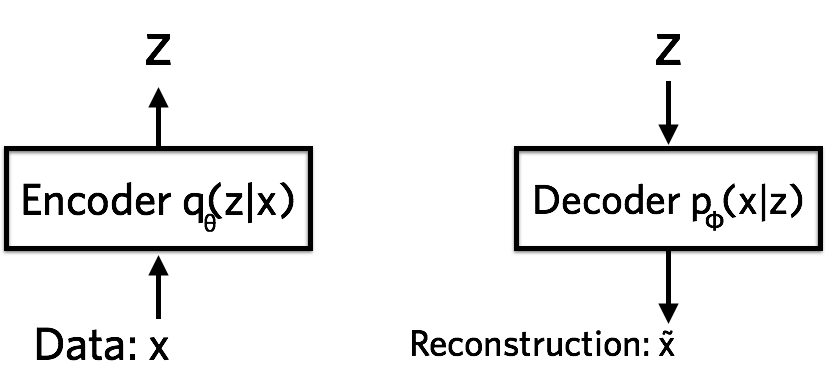
\includegraphics[width=\linewidth]{encoder-decoder.png}
    \caption{Simplified schematic of the encoder and decoder, where the left and right rectangles labelled $q(z|x)$ and $p(x|z)$ refer to the inferential and generative networks, respectively. First, $\vz$ is generated from $\vx$ using the encoder and then $\vx$ is reconstructed using $\vz$ \cite{jaanTutorial}. Note: the notation in this figure is opposite to what we use in this paper: $\theta$ and $\phi$ have been flipped such that $\theta$ parameterizes $q$ and $\phi$ parameterizes $p$. Otherwise, the setup is the same to what we have been discussing.}
    \label{fig:encoder-decoder}
\end{figure}

\subsection{The reparameterization trick}

A further advantage of amortisation via the encoder and decoder neural networks is that it allows us to convert this problem from one of sampling from a posterior distribution -- which can require the use of computationally intensive or mathematically complex methods such as expectation-maximization -- to a simple non-convex optimization problem. That is, all the terms in the ELBO loss function can be expressed in terms of $\phi$ and $\theta$, meaning that if we can differentiate through all the operations involved, then this problem can be solved with gradient descent. To revisit, the encoder and decoder form a single algorithm:
\begin{enumerate}
    \item Given $\vx$, compute $\vmu, \Sigma = g_\phi(\vx)$
    \item Sample $\vz\sim\N(\vmu,\Sigma)$
    \item Compute reconstruction $\hat{x} = f_\theta(\vz)$
\end{enumerate}

The one operation that does not allow for easy differentiation is the sampling step (2). In order to get around this, we use the ``reparameterization trick''. Recall that a $d$-dimensional isotropic Gaussian random variable can be converted into a sample from the $d$-dimensional multivariate normal distribution:
\[
    \vec{\epsilon} = (\vz - \vmu) \odot \frac{1}{\vsig} + \vmu
\]
Where $\vec{\epsilon}$ is a standard normal random variable (not to be confused with $\vz$, which is our latent variable with mean $\mu$ and covariance $\Sigma$) and $\vsig$ is the $d$-dimensional vector of standard deviations for the components of $\vz$. $\odot$ represents element-wise multiplication. Using simple algebra, we can rearrange this:
\[
    \vz = (\vec{\epsilon} \odot \vsig) + \vmu
\]
This means that sampling $\vz\sim\N(\vmu,\Sigma)$ is equivalent to sampling $\vec{\epsilon}\sim\N(0,I)$ and then transforming it into $\vz$ as above. The gradient operation is well-defined for sampling from the standard normal, so we can make the entire VAE algorithm differentiable by adding this reparameterization step:

\begin{enumerate}
    \item Given $\vx$, compute $\vmu, \Sigma = g_\phi(\vx)$. Let $\vsig = \sqrt{\operatorname{diag}(\Sigma)}$
    \item Sample $\vec{\epsilon}\sim\N(0, I)$
    \item Let $\vz = \vec{\epsilon}\odot\vsig + \vmu$
    \item Compute reconstruction $\hat{x} = f_\theta(\vz)$
\end{enumerate}


\subsection{$\beta$-VAE}

In the original paper, the authors provide a derivation of the $\beta$-VAE loss using constrained optimization \cite{higgins2016beta}. Given data $\vx$ distributed according to the data distribution $\D$, the goal is to jointly learn generative parameters $\theta$ and latent parameters $\phi$ for the distributions $\ptheta$ and $\qphi$, respectively. We want to find $\theta$ and $\phi$ such that the posterior log-probability $\ptheta(\vx|\vz)$ where $\vz\sim\qphi$ is maximized:
\begin{align*}
    \theta^*,\phi^* = \underset{\theta,\phi}{\argmax}\E_{\vx\sim\D}\left[ \Eq\left[ \log\ptheta\left( \vx|\vz \right) \right] \right]
\end{align*}
Subject to constraint
\begin{align*}
    \kl\left( \qphi(\vz|\vx)||p(\vz) \right) < \delta
\end{align*}
Where $\delta$ is a small positive constant (since KL divergence is nonnegative). The constraint is imposed to narrow the "information bottleneck" by encouraging the latent posterior $\qphi(\vz|\vx)$ to be close to a simple prior $p(\vz)$, which in this case is a standard gaussian, $\N(0, I)$. The idea is that we want to make $\qphi$ less expressive, which in turn forces it to be as efficient as possible in which latent factors are represented. Hopefully, the efficiency is maximized when the latent factors line up with the original factors that generated the data.

We can rewrite this constrained optimization problem as a Lagrangian subject to the KKT condition, with Lagrange multiplier $\beta$ and Lagrangian objective $\F$:

\begin{align*}
    \F(\theta, \phi, \beta; \vx, \vz) &= \Eq\left[ \log\ptheta(\vx|\vz) \right] - \beta\left( \kl(\qphi(\vz|\vx)||p(\vz)) - \delta \right) \\
    &= \Eq\left[ \log\ptheta(\vx|\vz) \right] - \beta\left( \kl(\qphi(\vz|\vx)||p(\vz))\right) + \beta\delta \\
    &\geq \Eq\left[ \log\ptheta(\vx|\vz) \right] - \beta\left( \kl(\qphi(\vz|\vx)||p(\vz))\right)
\end{align*}
Immediately, we can recognize that this is nearly identical to the vanilla VAE loss, except for the hyperparameter $\beta$. When $\beta=1$, this is equivalent to the vanilla VAE loss. When $\beta = 0$, the model becomes similar to a non-variational auto-encoder, since the only objective is to faithfully reconstruct the data. As $\beta$ increases, the bottleneck in the latent space becomes narrower, promoting a sparser latent representation (i.e. a latent space that more closely resembles a standard Gaussian).

\subsubsection{Measuring disentanglement}

The authors of the original $\beta$-VAE paper go a step further and propose a ``disentanglement metric'' to quantify how well the model's latent representations align with the hypothesized generative factors for the data \cite{higgins2016beta}.

Formally, we assume the data $\vx$ are drawn from a dataset $\D=\{X, V, W\}$, where $X$ is the data matrix, and $V, W$ are matrices of hypothesized {\it generative factors} for each data point. For instance, a factor for a dataset of faces might be {\it skin tone} or {\it glasses}. An image is created using a simulator: $\vx\sim\Sim(\vv, \vw)$. Then,
\begin{enumerate}
    \item Uniformly sample factor $y$ from the set of $K$ possible generative factors
    \item Repeat $L$ times:
    \begin{enumerate}
        \item Sample two sets of generative latent representations, $\vv_{1,l}$ and $\vv_{2,l}$ such that both $\vv_{1,l}$ and $\vv_{2,l}$ have the same value for factor $y$ and are free to differ in all other generative factors
        \item Simulate an image $x_{1,l\sim\Sim(v_{1,l})}$ and compute the latent representation $\vz_{1,l}\sim q(\vz|\vx_{1,l})$ using the encoder $g_\phi(\vx_{1,l})$. Repeat for $v_{1,l}$
        \item Compute a difference vector $z^l_{\diff}=|z_{1,l}-z_{2,l}|_1$
    \end{enumerate}
    \item Given all $z^l_{\diff}$ computed as above, calculate the average difference vector $\bar{z}_{\diff} = \frac{1}{L}\sum_{l=1}^Lz^l_{\diff}$
    \item Use $\bar{z}_{\diff}$ as the input for a linear classifier (i.e. logistic regression), where the goal is to predict the factor $y$ that was kept constant between all pairs of latent factors
\end{enumerate}

This algorithm can be seen in figure \ref{fig:disentanglement-metric}

\begin{figure}
    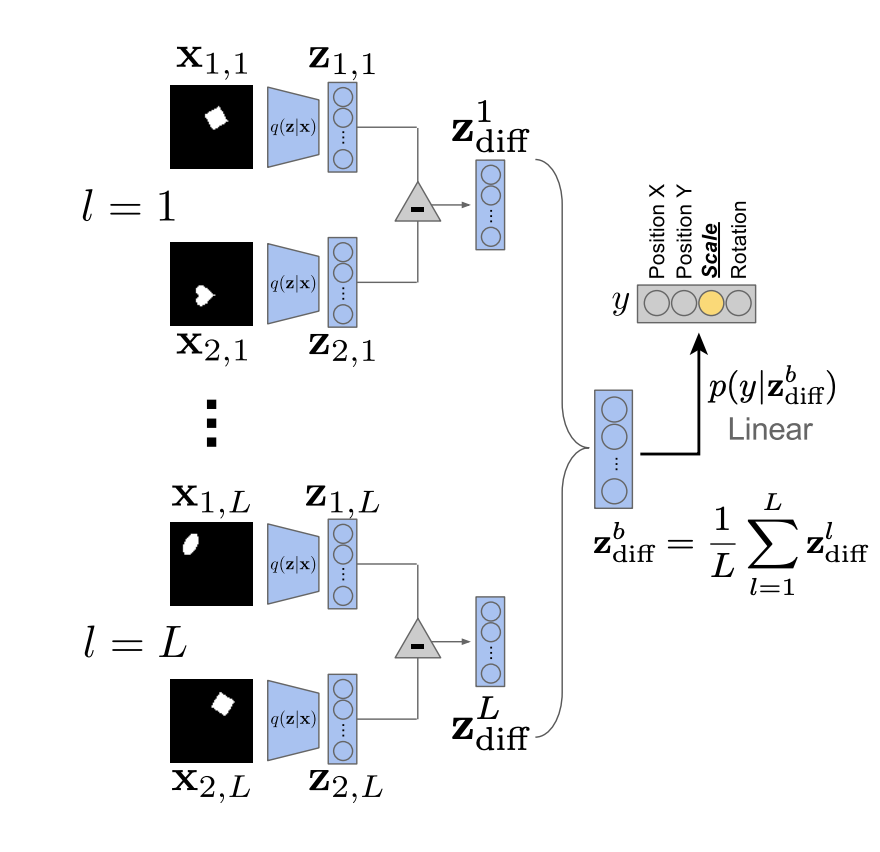
\includegraphics[width=\linewidth]{disentanglement-metric.png}
    \caption{A schematic of the proposed disentanglement metric from \cite{higgins2016beta}. Each vector $\vz^l_{\diff}$ in the process is generated from pairs of latent representations $z_{1,l}, z_{2,l}$ with the exact same value for a chose generative factor $y$. All of the $L$ pairs in batch $b$ may differ in terms of the value of the generative factor, but the choice of $y$ is constant between pairs. The linear classifier, $p(y|\vz^b_{\diff})$ is a multivariate classification algorithm whose goal is to predict which generative factor was used to generate the average difference vector $\vz_{\diff}^b$ (in the text, we refer to this average difference vector as $\bar{z}_{\diff}$).}
    \label{fig:disentanglement-metric}
\end{figure}

\subsection{Implementation}

Depending on the type and complexity of the data, various architectures for the inference and generative networks are used. In the simplest case, each is a feed-forward neural network, which is common for either numeric data or small-sized image data (e.g. MNIST, which is $28\times28\times1$). For larger image data, such as the CelebA dataset ($64\times64\times3$), convolutional neural networks (CNNs) are often used, with the structure of the generative network (often referred to as the "encoder") mirroring the structure of the inference network (often referred to as the "decoder"). The weights of the generative and inference networks are found using well-known gradient descent algorithms (e.g. the authors use Adam, RMSProp, and Adagrad for different experiments).